\documentclass{article}
\usepackage{listings}
\usepackage{xcolor}

\definecolor{codegreen}{rgb}{0,0.6,0}
\definecolor{codegray}{rgb}{0.5,0.5,0.5}
\definecolor{codepurple}{rgb}{0.58,0,0.82}
\definecolor{backcolour}{rgb}{0.95,0.95,0.92}

\lstdefinestyle{mystyle}{
    backgroundcolor=\color{backcolour},   
    commentstyle=\color{codegreen},
    keywordstyle=\color{magenta},
    numberstyle=\tiny\color{codegray},
    stringstyle=\color{codepurple},
    basicstyle=\ttfamily\footnotesize,
    breakatwhitespace=false,         
    breaklines=true,                 
    captionpos=b,                    
    keepspaces=true,                 
    numbers=left,                    
    numbersep=5pt,                  
    showspaces=false,                
    showstringspaces=false,
    showtabs=false,                  
    tabsize=2
}

\lstset{style=mystyle}
\usepackage[margin=1.5in]{geometry}
\setlength{\parskip}{1em}
\usepackage{hyperref}
\usepackage{graphicx}


\title{Use Case 3}
\author{Gabriel D Hofer}
\date\today

\begin{document}
\maketitle
%-------------------------------
%	ASSIGNMENT
%-------------------------------



1. Load data and create spark data frame
\lstinputlisting[language=Scala]{code/one.m}

2. Give marketing success rate. (No. of people subscribed / total no. of entries)
\lstinputlisting[language=Scala]{code/two.m}

3. Check max, min, Mean and median age of average targeted customer
\lstinputlisting[language=Scala]{code/three.m}

4. Check quality of clients by checking average balance, median balance of clients
\lstinputlisting[language=Scala]{code/four.m}

5. Check if age matters in marketing subscription for deposit
\lstinputlisting[language=Scala]{code/five.m}
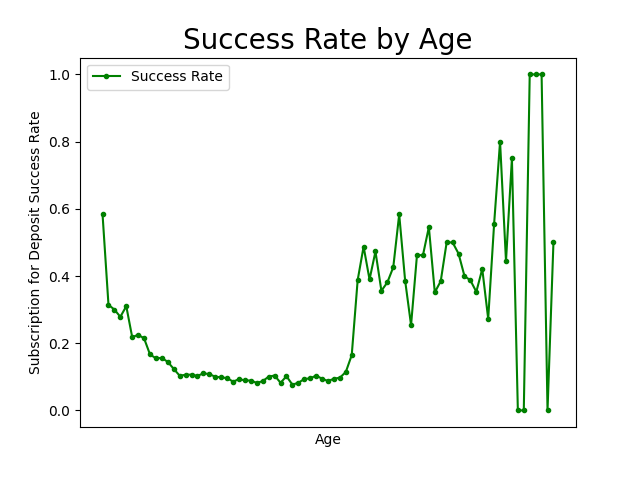
\includegraphics[scale=0.85]{images/success_rate_by_age.png}
\newpage
As seen from the data and the plot, the success rate increased significantly after age 61.
The success rate is also higher for people in the age range 18-29.

6. Check if marital status mattered for subscription to deposit.
\lstinputlisting[language=Scala]{code/six.m}
It appears that the Single category had a higher subscription success rate. 

7. Check if age and marital status together mattered for subscription to deposit scheme
\lstinputlisting[language=Scala]{code/seven.m}
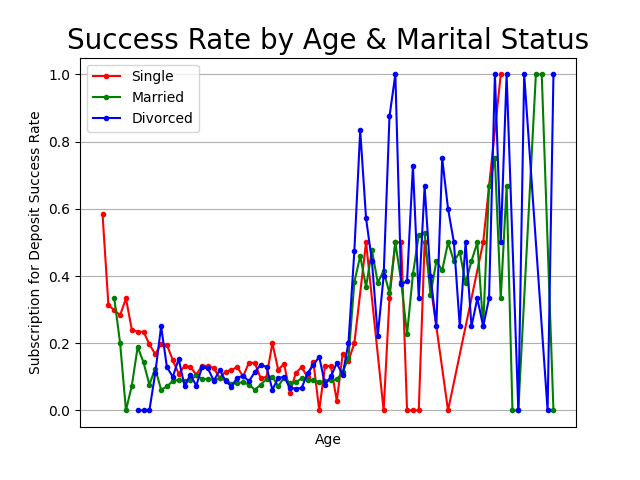
\includegraphics[scale=0.85]{images/age_marital.png}

As seen from the data and the plot, we can conclude that age and marital status both mattered for subscription to deposit scheme.

\end{document}
